\section{Full protocol and reproducibility}

\paragraph{Candidate construction.} Each non-empty trace in a held-out task group is a query. The gallery contains every other trace in the same benchmark and held-out fold, including both Human and Agent records. Query self-matches are removed by trace ID. A relevant candidate shares the benchmark-qualified task ID. Ties receive expected metric credit under a uniform random ordering. The random \Hit{} is the mean reciprocal gallery size at the query level, aggregated with equal benchmark weight.

\paragraph{Feature and training separation.} The input representation consists of normalized command names and coarse action labels derived by the pinned corpus parser. The association pair labels use only benchmark/task identity. The mode classifier trains on command TF--IDF unigram and bigram features. For training pairs, execution-mode features are generated by task-grouped inner cross-fitting; the outer held-out fold is not used to fit vocabulary, classification models, or the ranker. Candidate inclusion never depends on predicted or true mode.

\paragraph{Uncertainty.} Each reported interval resamples benchmark-qualified task groups within benchmark strata 5,000 times, preserving paired method comparisons and equal weighting of the three benchmarks. The intervals are conditional on each fixed task split and fitted model. Alternate seeds reuse the same traces and test split sensitivity; they are not independent samples or external replication.

\begin{table}[t]
\centering
\caption{Mode-aware minus task-supervised behavior \Hit{} change by task split.}
\label{tab:split-sensitivity}
\small
\rowcolors{2}{PaleGray}{white}
\begin{tabularx}{0.87\linewidth}{>{\raggedright\arraybackslash}Xrr}
\toprule
\rowcolor{InkBlue}\textcolor{white}{Split seed} & \textcolor{white}{Change} & \textcolor{white}{95\% task-cluster CI} \\
\midrule
20261030 (primary) & +0.0358 & [+0.0056, +0.0690] \\
20261130 & +0.0014 & [−0.0272, +0.0326] \\
20261230 & −0.0062 & [−0.0407, +0.0245] \\
20261330 & −0.0074 & [−0.0425, +0.0226] \\
20261430 & −0.0079 & [−0.0601, +0.0452] \\
20261530 & −0.0160 & [−0.0437, +0.0056] \\
\rowcolor{PaleBlue}\textbf{Alternate-split mean} & \textbf{−0.0072} & \textbf{[−0.0264, +0.0115]} \\
\bottomrule
\end{tabularx}
\end{table}

\begin{figure}[t]
\centering
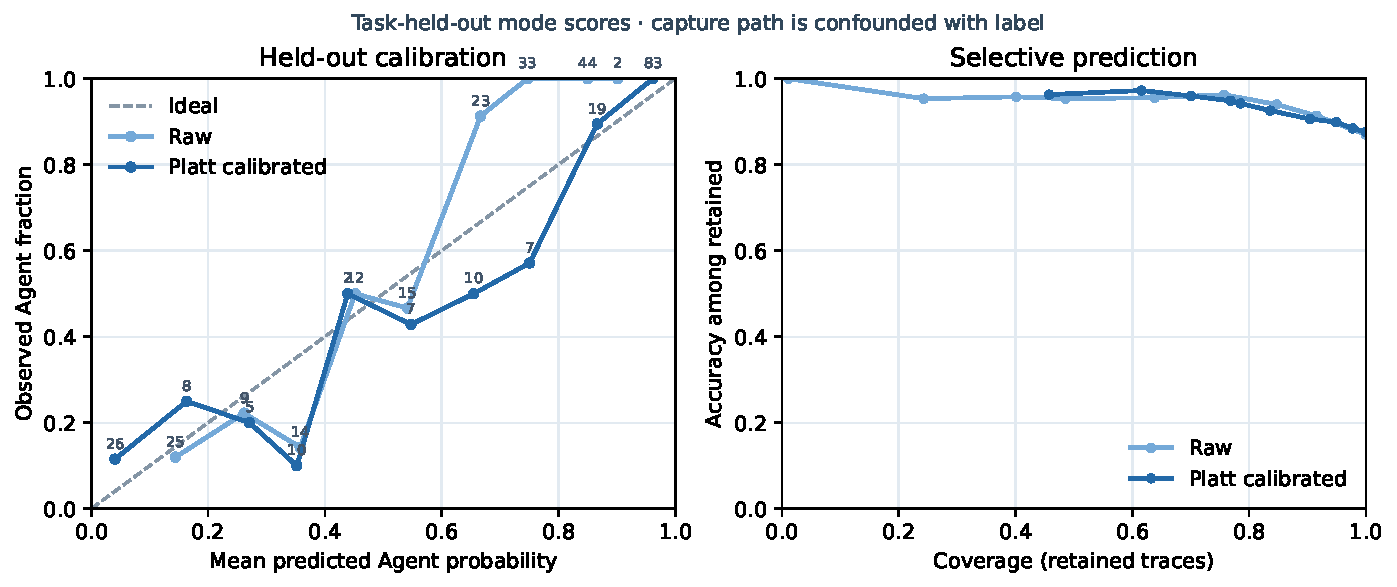
\includegraphics[width=\linewidth]{mixed_gallery_calibration.pdf}
\caption{Out-of-fold calibration and selective-prediction diagnostics. Scores describe Human/Agent record labels in the source release; capture path is confounded with the label.}
\label{fig:calibration}
\end{figure}

\paragraph{Data source and license.} Cyber Task Horizons is pinned to commit \texttt{178c0da1800f9c07311e1b8d6c61dd8104e7b4ae} under CC BY 4.0. The manifest records selected source files, hashes, suite and task IDs, collection labels, and latest-attempt deduplication. Raw traces are fetched locally and are not redistributed by this repository. Task identity provides a same-challenge retrieval proxy only.

\paragraph{Reproduction.} From the repository root, install the locked CPU dependencies, download the pinned public traces, then run:

\begin{verbatim}
.venv/bin/python scripts/run_mixed_gallery.py --bootstraps 5000
.venv/bin/python -m unittest discover -s tests -v
\end{verbatim}

The run writes \texttt{results/mixed\_gallery.json}, task/query CSVs, held-out mode predictions, and three PDF/PNG figures. The experiment and drawing implementation is retained in \texttt{scripts/run\_mixed\_gallery.py}; the executable notebook is \texttt{notebooks/07\_mixed\_gallery.ipynb}. The JSON records the data revision, protocol version, split seeds, evaluation definition, bootstrap method, and script hash.
